\chapter{Оптика}
\thispagestyle{empty}
\clearpage
\begin{problem}
Установка (см. рисунок) состоит из лампы накаливания, ёмкости, заполненной бензолом, две противоположные стенки которой сделаны из исландского шпата так, что в состоянии покоя не пропускают свет лампочки и двух металлических пластин с выводами, приложенных к горизонтальным граням ёмкости. Объяснить, почему при прикладывании к пластинам напряжения свет начинает беспрепятственно проходить через установку.
{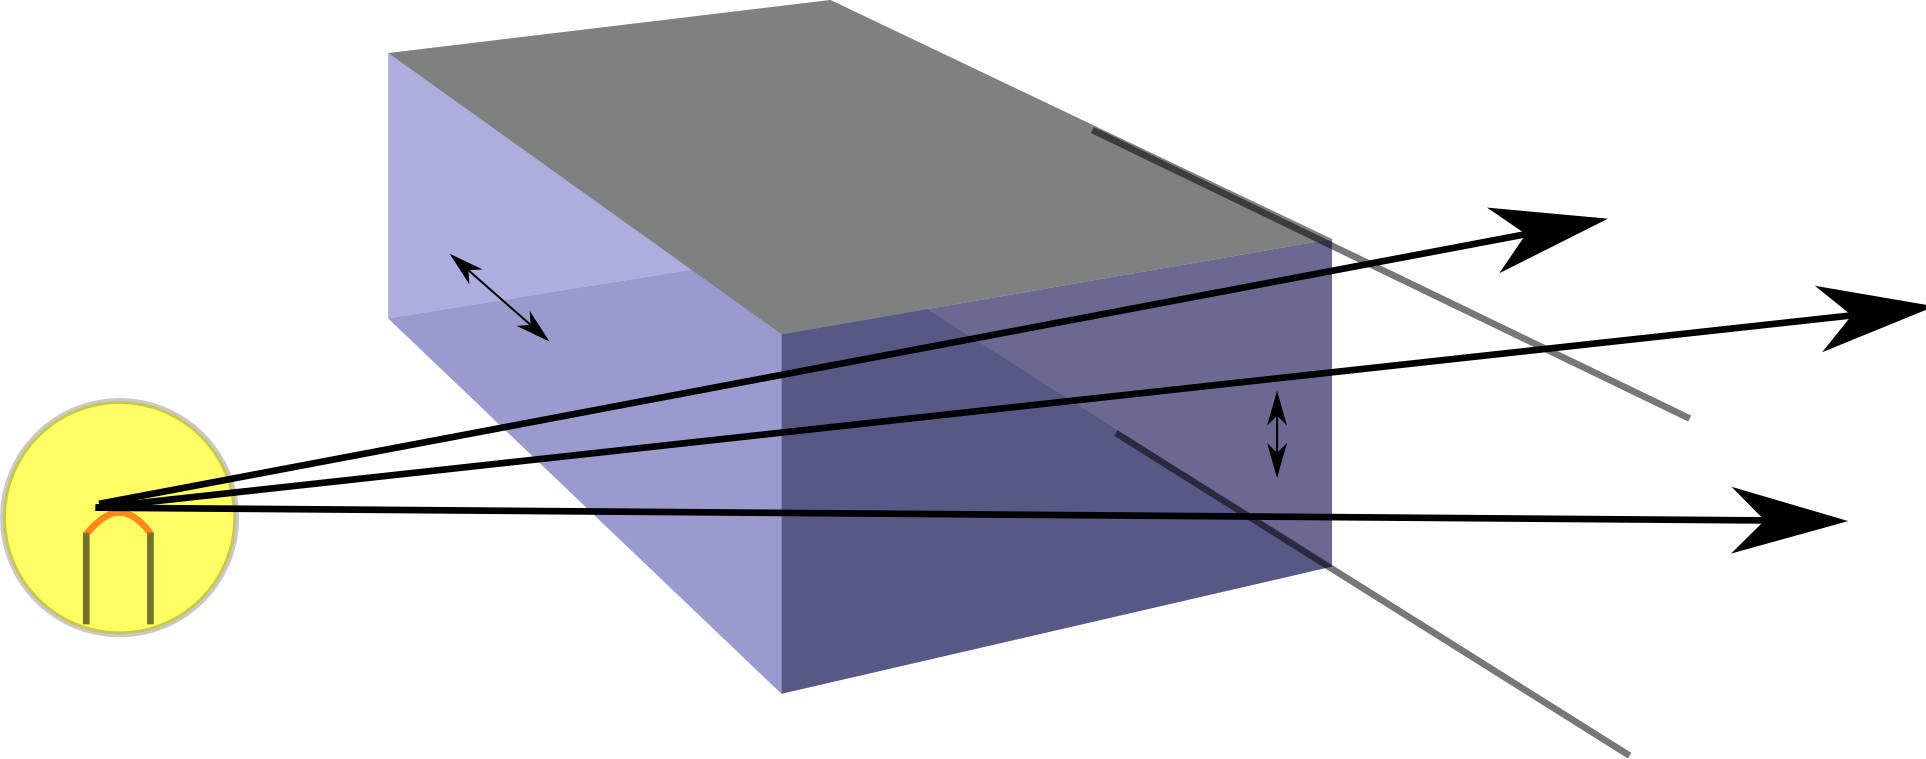
\includegraphics[width=0.8\textwidth]{./kerr}}
\end{problem}
\begin{problem}
Придумайте способ получения циркулярно поляризованной волны в радиочастотном диапазоне, используя лишь эктронные компоненты.
\end{problem}
\begin{problem}
Известно, что у большинства веществ, например у стекла, магнитная и электрическая проницаемость положительны. Особый интерес в оптике представляет плазма, так как на частотах меньше собственной\footnote{см. умную книжку} электрическая её проницаемость меньше нуля. Однако, уравнения Максвелла и уравнения связи не теряют смысл и при одновременной отрицательности как магнитной, так и электрической проницаемостей вещества. Начертите картину прохождения лучей света через двояковогнутую линзу из вещества с $\varepsilon<0$ и $\mu<0$ одновременно. Попытайтесь найти другие интересные свойства таких веществ.
\end{problem}